\chapter{Introduction}
\label{sec:introduction}
%\chapter{Einleitung}
%\label{sec:einleitung}

One of the key challenges on the way towards autonomous robot navigation is localization. To achieve any autonomous task, a robot needs to estimate its pose, which is the robot position and orientation in space. Visual-inertial Localization is one approach to estimate the robots pose by combining the information of an inertial measurement unit (IMU) and the information of a camera. A camera image provides rich structure information about a scenery and the IMU measurements help estimating the robot pose over short distances. Due to these complementary properties a camera-IMU sensor system is well suited for the complex task of robot localization. The visual-inertial approach has some key advantages comparing with approaches using other information sources like laser range finders or external localization systems: A) Camera and IMU are lightweight sensors, which can be equipped on a flying robot, B) Camera and IMU are passive sensors with a small energy consumption and C) Visual-inertial localization relies solely on onboard sensors, therefore it can be applied in GPS-denied environments without modifying the environment itself. \\


\begin{figure}[h]
   \centering
   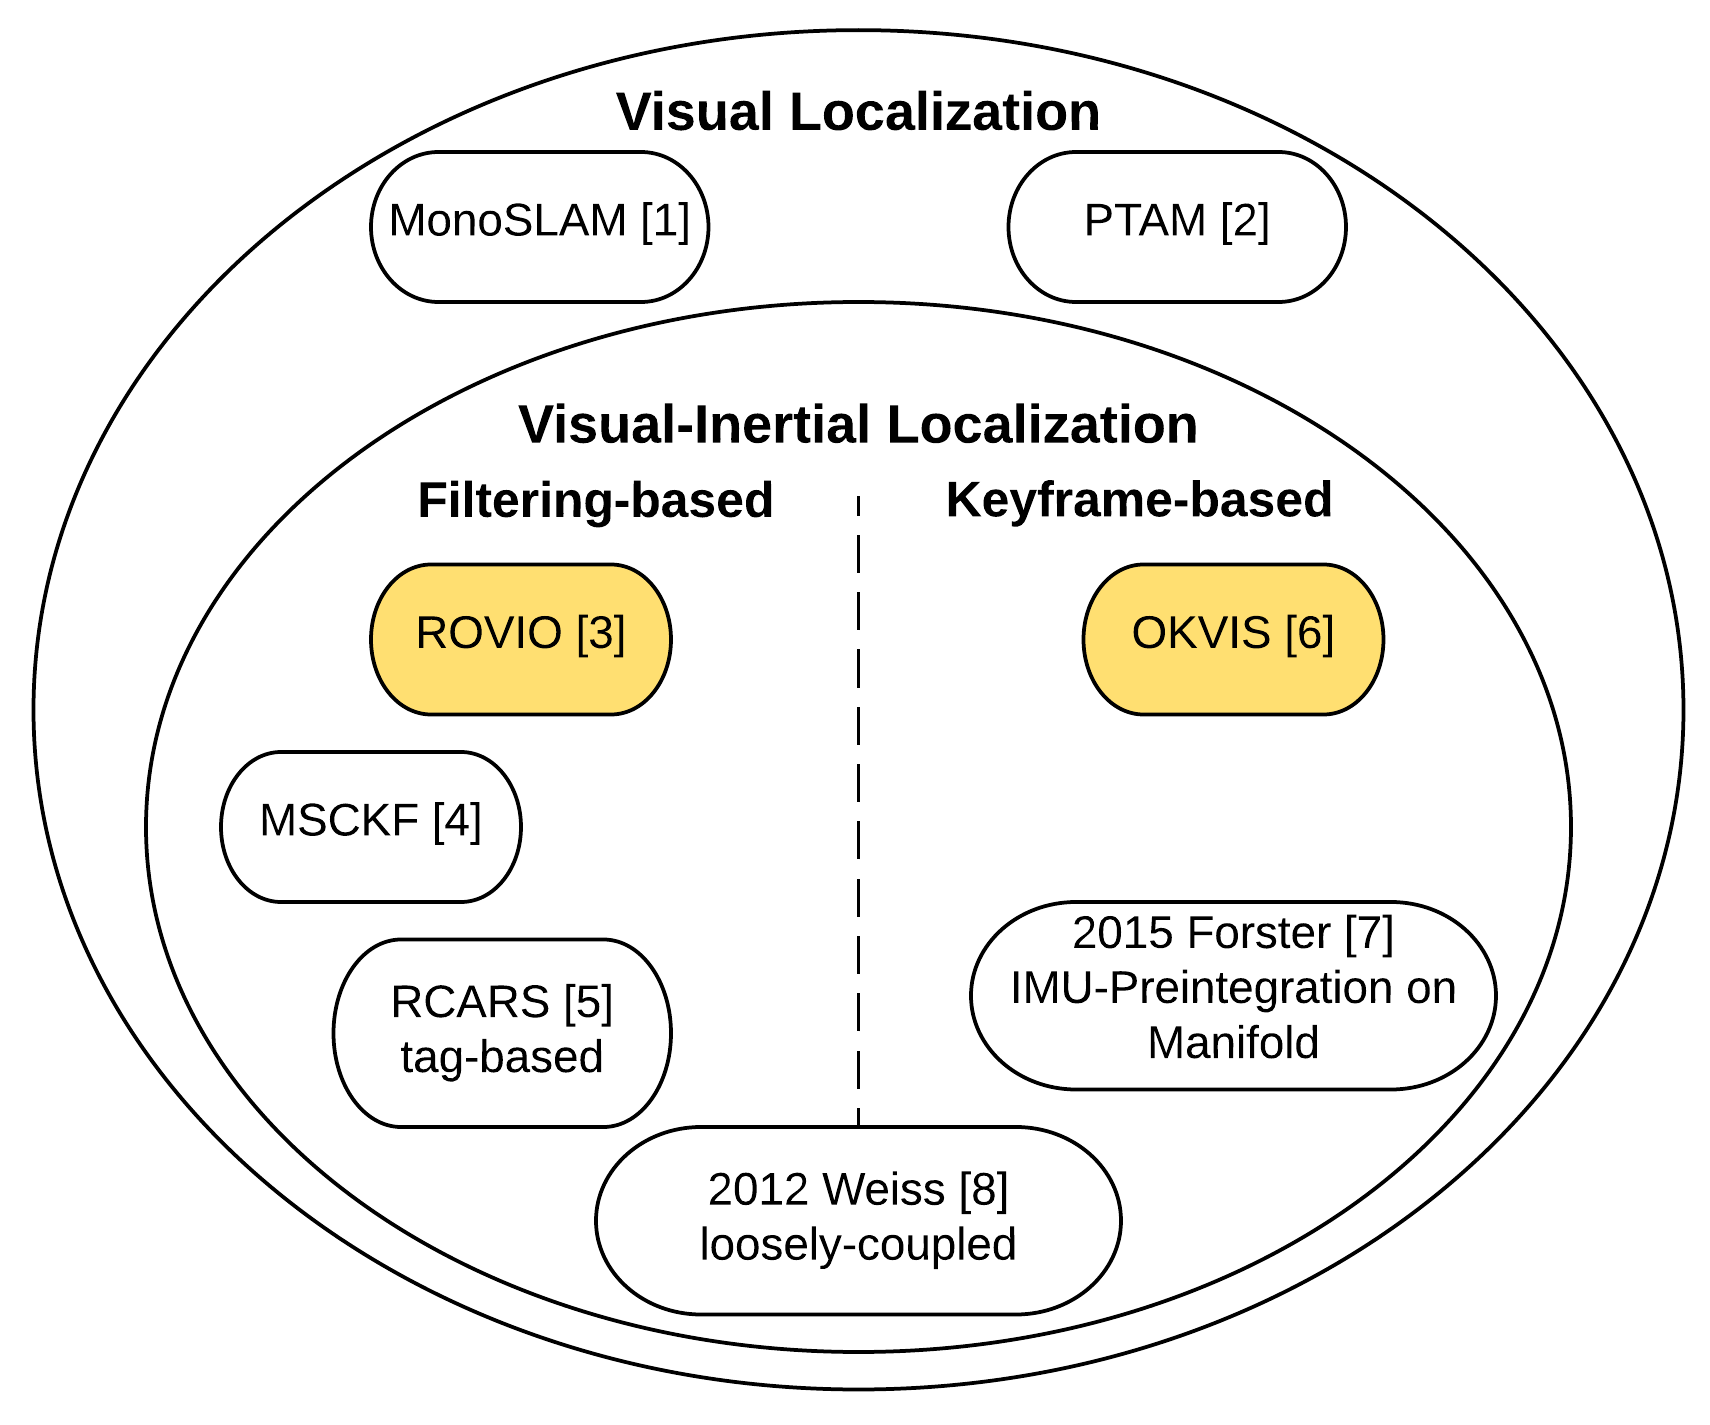
\includegraphics[width=0.5\textwidth]{images/state_of_the_art.png}
   \caption{The field of visual localization and the subfield of visual-inertial localization with important published algorithms.}
   \label{pics:state_of_the_art}
\end{figure}
% SVO \cite{forster2014svo}
% LSD-SLAM \cite{engel2014lsd}

Over the last Decade a series of different implementations achieving visual-inertial robot localization have been proposed. Figure \ref{pics:state_of_the_art} shows an overview of the field of visual localization and the visual-inertial localization in particular. Pioneer work has been achieved with MonoSLAM (Davison et al. \cite{davison2007monoslam}), introducing a framework for simultaneous localization and mapping (SLAM) based on a single camera that is running in real-time, and PTAM, Parallel Tracking and Mapping (Klein et al., \cite{klein2007parallel}), achieving an enhancement regarding computational complexity by parallelizing the mapping and tracking functionalities into two separate threads. \\

Visual-inertial localization can be divided into the principally different filtering-based and keyframe-based approaches,  see figure \ref{pics:filtering_keyframe}. The filtering-based approach (figure \ref{pics:filtering_keyframe} a) achieves robot localization by propagation of the estimated pose based on the IMU measurements and updating this prior belief based on the camera observation. In the filtering-based approach an estimation in the past will never be corrected based on a new observation. Because of this property, filtering-based algorithms are tendentious more prone to drift, but computationally less expensive than the keyframe-based implementations. ROVIO, robust visual-inertial odometry (Blösch et al., \cite{bloeschrobust}) is a recent and promising implementation of the filtering-based approach using an extended kalman filter (EKF) and direct intensity image patches. Other promising filtering-based algorithms include MSCKF, a multi-state constraint kalman filter (Mourikis et al., \cite{mourikis2007multi}), who introduced a filter working on the information of a set of past frames and RCARS, robot-centric absolute reference system (Neunert et al., \cite{neunert2015open}), who demonstrated a filtering-based localization system for a scenery with artificial tags included.

The keyframe-based approach (figure \ref{pics:filtering_keyframe} b) achieves robot localization by a nonlinear optimization based on both the camera and IMU information. OKVIS, optimal keyframe-based visual inertial SLAM (Leutenegger et al., \cite{leutenegger2015keyframe}) is one very promising implementation of this approach, which includes both the camera and IMU information into a single error function. Another recently published and promising implementation applies a direct approach with preintegration of the IMU measurements (Forster et al., \cite{forster2015imu}).

In addition to the filtering-based and keyframe-based approach, an implementation has been proposed that combines the two approaches in a loosely-coupled way by performing a keyframe-based implementation on the vision side and fusing the result afterwards in a filter with the IMU information (Weiss et al., \cite{weiss2012real}). \\

\begin{figure}
  \begin{subfigure}[b]{0.4\textwidth}
    \captionsetup{skip=6pt}
    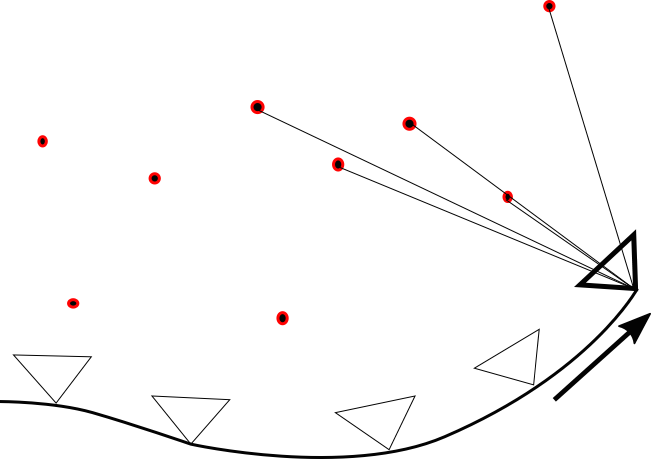
\includegraphics[width=\textwidth]{images/filteringbased_2.png}
    \caption{filtering-based}
    \label{fig:1}
  \end{subfigure}
  \hfill
  \begin{subfigure}[b]{0.4\textwidth}
    \captionsetup{skip=6pt}
    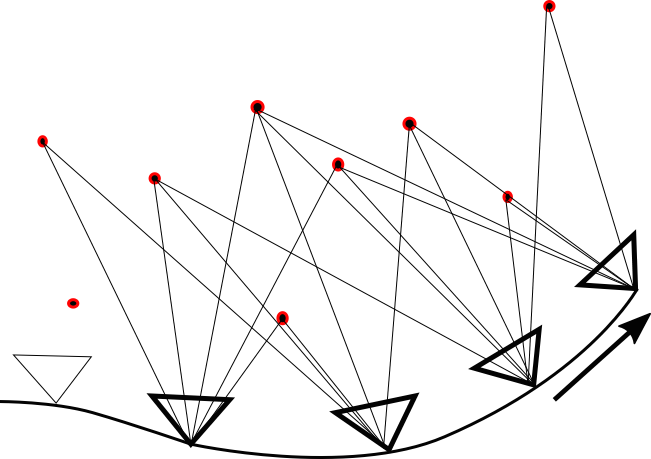
\includegraphics[width=\textwidth]{images/keyframebased_2.png}
    \caption{keyframe-based}
    \label{fig:2}
  \end{subfigure}
\caption{(a) shows the filtering-based principle of localization: The robot pose is propagated between two camera frames based on the IMU measurements and updated based on the cameras landmark observations. The pose of a past frame is not corrected based on a new observation. (b) shows the keyframe-based approach to localization: The robot pose is estimated by a nonlinear optimization based on the IMU data and the landmark observations of a \textit{set} of frames. With this approach the pose of a past frame will be corrected based on a new observation.}
\label{pics:filtering_keyframe}
\end{figure}

It is already known since a few years that the keyframe-based approach is preferable to the filtering-based approach whenever the computational resources are available (Strasdat et al., \cite{strasdat2010real}). Nevertheless, the ongoing research in both domains, the superior performance regarding computational complexity and the availability and robustness of filtering-based implementations show the significance of the filtering-based approach untill today as well. \\

This work presents a direct comparison of the filtering-based implementation ROVIO and the keyframe-based implementation OKVIS on real data. Both algorithms show promising results, have been developed at ETH Zurich and are on the way of being published open source. Section \ref{sec:rovio} and \ref{sec:okvis} introduce the characteristics, working principles, and differences of ROVIO and OKVIS, respectively. Section \ref{sec:metrics} introduces the evaluation metrics and presents a differentiation between global and local accuracy. The results and their discussion can be found in section \ref{sec:results}: Section \ref{sec:ijrr} contains the comparison based on indoor data collected with a hardware-wise time synchronized sensor system and section \ref{sec:euroc} gives some deeper insights into the ROVIO performance on a complementary dataset. For a wide number of applications it will be of interest whether an implementation of visual-inertial localization can work on a generic sensor system. An experimental analysis approaching the question if ROVIO is able to work with a generic sensor system is found in section \ref{sec:timesync}. \\
